% \setcounter{section}{0}
\section{Логика и арифметика}

\subsection{Любую булеву функцию можно выразить формулой в КНФ или в ДНФ.}

\begin{center}
    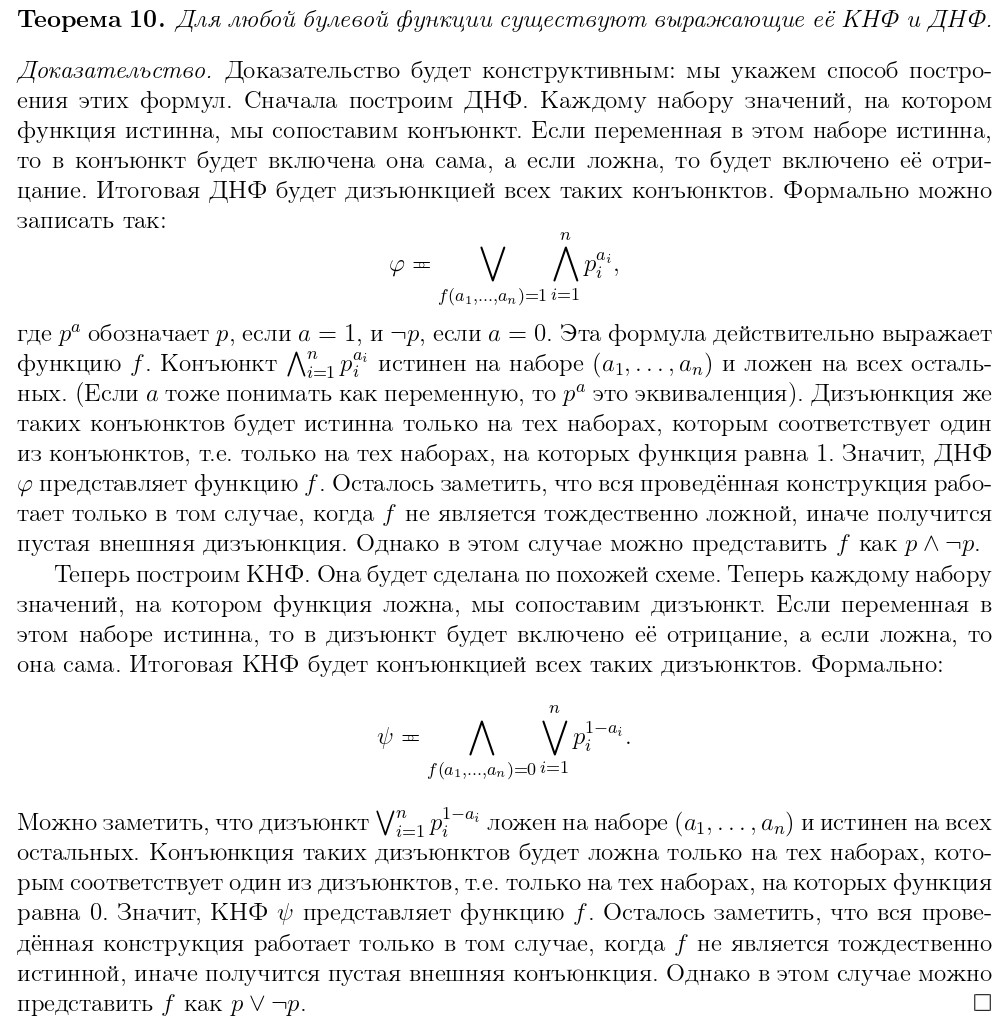
\includegraphics[width=0.95\linewidth]{images/1_propositions_knf}
\end{center}

\subsection{Замкнутость классов Поста относительно композиции.}

\textbf{Определение:} суперпозиция функций из множества $F$:
\begin{itemize}
    \item Суперпозициz порядка 0 -- все проекторы, т.е. функции вида $pr_i(p_1,\ldots,p_n)=p_i$
    \item Суперпозиция порядка $m+1$ -- функция вида $h(p_1,\ldots,p_n)=f(g_1(p_1,\ldots,p_n),\ldots,g_k(p_1,\ldots,p_n))$, где $f\in F$, $f$ зависит от $k$ аргументов, $g_1,\ldots,g_k$ - суперпозиции порядка $\leqslant m$, хотя бы одно из них в тоности $m$.
\end{itemize}

\textbf{Определение:} Замыкание класса $F$ -- множество всех суперпозиций всех порядков функции из $F$ (Обозначение: $[F]$)
\textbf{Определение:} Класс замкнут, если $[F]=F$
\newline \par Докажем замкнутость классов Поста для $f \in T_1,T_0,S,M,L$:
\begin{itemize}
    \item $[T_1] = T_1: \;\; h(1,\ldots,1)=f(g_1(1,\ldots,1),\ldots,g_k(1,\ldots,1))=f(1,\ldots,1)=1$
    \item $[T_0] = T_0: \;\;$ аналогично $T_1$
    \item $[M] = M: \;\; 
            \left\{
              \begin{array}{ccc}
                    x_1\leqslant y_1\\
                    \ldots \\
                    x_n\leqslant y_n
              \end{array}
            \right\} \Rightarrow 
            \left\{
              \begin{array}{ccc}
                    g_1(x_1,\ldots,x_n)\leqslant g_1(y_1,\ldots,y_n)\\
                    \ldots \\
                    g_k(x_1,\ldots,x_n)\leqslant g_k(y_1,\ldots,y_n)
              \end{array}
            \right\} \Rightarrow \newline
            f(g_1(x_1,\ldots,x_n),\ldots,g_k(x_1,\ldots,x_n)) \leqslant f(g_1(y_1,\ldots,y_n),\ldots,g_k(y_1,\ldots,y_n)) $
    \item $[S] = S: \;\; f(g_1(\neg p_1,\ldots,\neg p_n),\ldots,g_k(\neg p_1,\ldots,\neg p_n)) = f(\neg g_1(p_1,\ldots,p_n),\ldots,\neg g_k(p_1,\ldots,p_n)) = \neg f(g_1(p_1,\ldots,p_n),\ldots,g_k(p_1,\ldots,p_n))$
    \item $[L] = L: \;\; f(g_1(p_1,\ldots,p_n),\ldots,g_k(p_1,\ldots,p_n)) = p_{i_1}\oplus \ldots \oplus p_{i_m} \oplus\alpha\oplus\ldots\ldots\oplus p_{j_1}\oplus \ldots \oplus p_{j_q} \oplus\beta\oplus\gamma$, где $\alpha,\beta\gamma\in\{0,1\}$. После сокращения дублей получится выражение такого же вида.
\end{itemize}

\subsection{Вывод формулы вида $A \to A$ в исчислении высказываний.}
Доказательство приведено в определениях пункт 6). 

\subsection{Теорема о корректности исчисления высказываний.}
\textbf{Корректность ИВ:} Если $\vdash \phi$, то $\phi$ -- тавтология
\newline $\blacktriangle$ 1) Любая аксиома есть тавтология. Проверяется непосредственно по таблице истинности. 
\newline 2) Правило MP тоже корректно: если $A$ и $A \to B$ всегда истинны, то $B$ тоже всегда истинно. $ \blacksquare$

\subsection{Сведение задачи о выполнимости произвольной формулы к задаче о выполнимости 3-КНФ.}
\textbf{Утверждение:} Пусть $\phi$ -- КНФ. Тогда выполнимость $\phi$ эквивалентна выполнимости $\phi'$, образованной следующим образом: каждый дизъюнкт $(l_1 \lor l_2 \lor \ldots \lor l_k)$ заменяется на такую КНФ: $(l_1 \lor x_1) \land (\neg x_1 \lor l_2 \lor x_2) \land\ldots\land (\neg x_{k-2} \lor l_{k-1} \lor x_{k-1}) \land (\neg x_k \lor l_k)$, где переменные $x_1, \ldots, x_k$ свои для каждого дизъюнкта.

$\blacktriangle$ Пусть $\phi$ выполнима. Тогда при выполняющем наборе один из литералов $l_1, \ldots, l_k$ истинен, например, $l_j$. Пусть тогда все $x_i$ с $i < j$ равны $1$, а все $x_i$ с $i \geqslant j$ равны $0$. Это сделает истинным все скобки в новой КНФ.

Пусть, напротив, выполнима $\phi'$. Каждая из переменных $x_i$ может сделать истинной ровно одну скобку. Значит, все они могут сделать истинными максимум $k - 1$ скобку. Оставшаяся должна стать истинной за счёт $l_j$. А значит, и исходный дизъюнкт выполнен. $\quad \blacksquare$


\subsection{Представление задачи о раскраске графа и задачи о расстановке ферзей на шахматной доске как задачи о выполнимости КНФ.}
\begin{itemize}
    \item \textit{Задача о 3-раскраске вершин графа.} Пусть задан некоторый неориентированный граф. Ставится вопрос: можно ли его вершины раскрасить в 3 цвета, так чтобы
    вершины одного цвета не были соединены ребром. КНФ строится так: для каждой вершины $i$ заводится две переменных $p_i$ и $q_i$. Будем считать, что пара значений
    $(0, 1)$ кодирует первый цвет, пара $(1, 0)$ второй цвет, а пара $(1, 1)$ третий цвет. Чтобы исключить вариант $(0, 0)$, добавим условия $(p_i \lor q_i)$. Далее, для каждого
    ребра $(i, j)$ пара $(p_i, q_i)$ должна отличаться от пары $(p_j, q_j)$. Это выражается такой КНФ: $$(p_i\lor p_j \lor q_i \lor q_j )\land(p_i\lor p_j \lor \neg q_i \lor \neg q_j )\land (\neg p_i\lor \neg p_j\lor q_i\lor q_j )\land(\neg p_i\lor \neg p_j \lor \neg q_i \lor\neg q_j )$$
    Выполнимость конъюнкции всех таких формул эквивалентна раскрашиваемости исходного графа.
    
    \item \textit{Задача о расстановке ферзей на шахматной доске.} Известна такая задача: можно ли расставить $8$ ферзей на шахматной доске, так чтобы они не били друг друга. Мы заведём переменные $p_{ij}$, истинность которых означает, что в клетке с координатами $(i, j)$ стоит ферзь. 
    \newline -- По условию в одной строке не может быть двух ферзей, значит, в каждой должен быть ровно один. Достаточно написать дизъюнкты вида $(p_{i1} \lor p_{i2} \lor \ldots\lor p_{i8})$. \newline -- Далее, запишем условия, что в каждом столбце стоит не более одного ферзя. А именно, для каждого набора $(i, j \neq i, k)$ возьмём дизъюнкт $(\neg p_{ik} \lor \neg p_{jk})$. Аналогичные условия для строк можно записать отдельно, но они будут следовать из уже написанных. \newline -- Также нужно написать условия для диагоналей: $(\neg p_{ij} \lor \neg p_{i+k,j+k})$ и $(\neg p_{ij} \lor\neg p_{i+k,j-k})$ при всех $i$, всех $j < 8$ и всех $k> 0$ (записываются только те условия, где все индексы попадают в интервал от 1 до 8). \newline Любой выполняющий набор для такой системы задаёт расстановку ферзей. Можно рассматривать разные варианты задачи: другой размер доски, фиксированное положение некоторых ферзей (тогда добавятся дизъюнкты $p_{ij}$) или запрещённые клетки (тогда добавятся дизъюнкты $\neq p_{ij}$).
\end{itemize}
В обоих случаях мы получили не 3-КНФ: в некоторых дизъюнктах больше трёх литералов.

\subsection{Теорема о корректности метода резолюций: из выполнимой КНФ нельзя вывести $\bot$.}
\textbf{Теорема:} Метод резолюций всегда заканчивает свою работу, причём для невыполнимых КНФ выводится $\bot$ (полнота), а для выполнимых не выводится (корректность). Таким образом, метод резолюций позволяет проверить выполнимость формулы: достаточно добавить все возможные резольвенты и проверить, встретился ли $\bot$.

$\blacktriangle$ Всего существует конечное число дизъюнктов, так что в какой-то момент новые перестанут появляться, поэтому метод всегда заканчивает свою работу. Как обычно, корректность доказывается легко. Действительно, если исходная КНФ была выполнима, то она останется выполнимой после добавления любого числа резольвент. Но КНФ с $\bot$ выполнимой быть не может. Значит, для выполнимой КНФ $\bot$ не появится. $\quad \blacksquare$


\textit{Пример:} Невыполнимая КНФ $(x_1 \lor x_2 \lor x_3) \land (\neg x_1 \lor x_2) \land (\neg x_2 \lor x_3) \land \neg x_3$ опровергается так:
\newline 1) $(x_1 \lor x_2 \lor x_3) \land (\neg x_1 \lor x_2) \Rightarrow (x_2 \lor x_3)$
\newline 2) $(x_2 \lor x_3) \land (\neg x_2 \lor x_3) \Rightarrow x_3$
\newline 3) $x_3 \lor \neg x_3 \Rightarrow \bot$

\subsection{Значение терма (формулы) первого порядка зависит только от значений его (её) параметров.}

\textbf{Теорема:} Истинность формулы (значение терма) зависит только от её (его) параметров. Иными словами, если оценки $\pi$ и $\rho$ таковы, что $\forall x \in $ Param$(\phi) \;
(\text{или }x \in $ Param$(t))$ выполнено $\pi(x) = \rho(x)$, то $[\phi](\pi) = [\phi](\rho) \; (\text{или }[t](\pi) = [t](\rho))$.
\newline $\blacktriangle$ Будем доказывать утверждение индукцией по построению терма, а затем формулы:
\begin{itemize}
    \item Если $t = x$, то $[t](\pi) = \pi(x) = \rho(x) = [t](\rho)$
    \item Если $t = c$, то $[t](\pi) = [c] = [t](\rho)$
    \item Если $t = f(t_1,\ldots, t_k)$, то в силу Param$(t_i) \subset$ Param$(t)$ по предположению индукции имеем $[t_i](\pi) = [t_i](\rho)$. Поэтому $[t](\pi) = [f]([t_1](\pi),\ldots, [t_k](\pi)) = [f]([t_1](\rho),\ldots, [t_k](\rho)) = [t](\rho)$;
    \item Если $\phi = P(t_1,\ldots, t_k)$, то рассуждение аналогично предыдущему;
    \item Если $\phi = \neg\psi$, то $[\phi](\pi) = \neg[\psi](\pi) = \neg[\psi](\rho) = [\phi](\rho)$. Здесь предположение индукции использовано во втором равенстве;
    \item Если $\phi = (\psi \land\gamma)$, то $[\phi](\pi) = [\psi](\pi) \land [\gamma](\pi) = [\psi](\rho) \land [\gamma](\rho) = [\phi](\rho)$. Здесь во втором равенстве использовано предположение индукции и вложения Param$(\psi) \subset$ Param$(\phi)$ и Param$(\gamma) \subset$ Param$(\phi)$. Случай $\phi = (\psi \lor\gamma)$ и $\phi = (\psi \to\gamma)$ разбираются аналогично;
    \item Если $\phi = \exists x\psi$, то ключевое соображение состоит в следующем: если $\pi(y) = \rho(y)$ для всех $y \in$ Param$(\psi) \setminus \{x\}$, то $\pi_{x\to m}(y) = \rho_{x\to m}(y)$ уже для всех $y \in$ Param$(\psi)$, в том числе для $y = x$. Действительно, $\pi_{x\to m}(y) = \rho_{x\to m}(y) = m$, а для $y\neq x$ равенство есть по предположению. Поэтому $[\phi](\pi) = \lor_{m\in M}[\psi](\pi_{x\to m}) = \lor_{m\in M}[\psi](\rho_{x\to m})=[\phi](\rho)$. Аналогичное рассуждение работает и для $\phi = \forall x\psi$. $\quad \blacksquare$
\end{itemize}

\subsection{Выразимость свойств «равняться нулю», «равняться единице», «делиться нацело», «быть простым числом», «равняться наибольшему общему делителю», «равняться наименьшему общему кратному» в интерпретации $\langle\mathbb{N},\cdot\;,=\rangle$.}

Рассмотрим интерпретацию $\langle\mathbb{N},\cdot\;,=\rangle$. Будем выражать в ней различные предикаты:
\begin{itemize}
    \item $x = 0 \; \Leftrightarrow \; \forall y \; x \cdot y = x$
    \item $x = 1 \; \Leftrightarrow \; \forall y \; x \cdot y = y$
    \item $x \svdots y \; \Leftrightarrow \; \exists z \; x= y \cdot z$
    \item $Prime(p) \; \Leftrightarrow \; (p\neq 1 \;\land\; \forall q(p\svdots q \to (q=1 \;\lor\; q=p)))$
    \item $d=$ НОД$(x,y) \; \Leftrightarrow \; (x\svdots d \;\land\; y \svdots d \;\land\; \forall k ((x\svdots k \;\land\; y \svdots k)\to d \svdots k))$
    \item $d=$ НОK$(x,y) \; \Leftrightarrow \; (d\svdots x \;\land\; d \svdots y \;\land\; \forall k ((k\svdots x \;\land\; k \svdots y)\to k \svdots d))$
    
\end{itemize}

\subsection{Любую формулу первого порядка можно привести к предваренной нормальной форме.}

\textbf{Определение:} Формула находится в предварённой нормальной форме, если вначале идут кванторы по некоторым переменным в некотором порядке, а затем — бескванторная формула.

\textbf{Теорема:} Для любой формулы существует эквивалентная ей формула в предваренной нормальной форме.

$\blacktriangle$ Алгоритм будет таким: сначала переименовать связанные переменные, так чтобы под всеми кванторами были разные переменные, притом не совпадающие с именами свободных переменных. Затем вынести все кванторы наружу, меняя их при выносе из отрицания или посылки импликации по правилам 4-7 из списка ниже. $\quad \blacksquare$
\newline
\newline
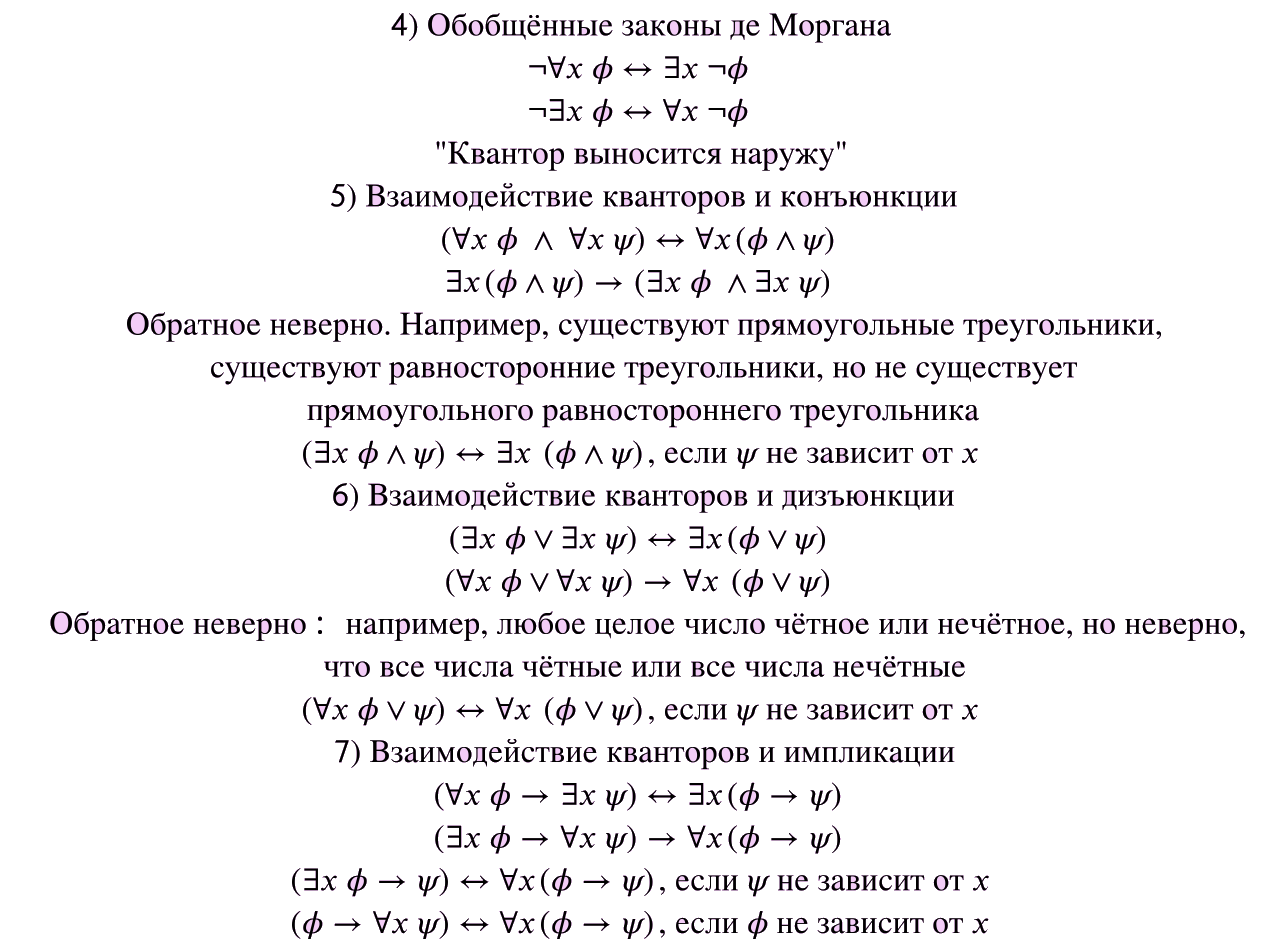
\includegraphics[width=0.9\linewidth]{images/1_propositions_rules}

\textit{Пример:} $\exists x A(x) \land \exists xB(x) \; \Leftrightarrow \; \exists x A(x) \land \exists yB(y) \; \Leftrightarrow \; \exists x (A(x) \land \exists yB(y)) \; \Leftrightarrow \; \exists x\exists y( A(x) \land B(x)) $

\subsection{Вывод правила обобщения в исчислении предикатов.}
Правило обобщения: $$\frac{\phi}{\forall x \;\phi}$$
$\blacktriangle$ 1) $\phi$ -- считаем, что уже вывели
\newline 2) $\psi$ -- некоторая аксиома, не зависящая от $x$
\newline 3) $\phi\to(\psi\to\phi)$ -- аксиома 1
\newline 4) $\psi\to\phi$ -- MP из 1 и 3
\newline 5) $\psi\to\forall x \phi$ -- 2-ое правило Бернайса
\newline 6) $\forall x \phi$ -- MP из 2 и 5 $\quad \blacksquare$

\subsection{Вывод формулы вида $\exists x \forall y \phi \to \forall y \exists x \phi$ в исчислении предикатов.}

Доказательство приведено в определениях пункт 12). 

\subsection{Любое совместное множество формул первого порядка непротиворечиво.}
$\blacktriangle$ От противного: пусть Г -- противоречиво. Если Г $\vdash \phi$ и все формулы из Г верны на некотором наборе (def: совместности), то $\phi$ верно на том же наборе. При этом Г $\vdash \phi$ и Г $\vdash \neg\phi$, то Г $\phi$ и $\neg\phi$ одновременно верны на этом наборе, противоречие $\Leftrightarrow$ Г -- непротиворечиво. $\quad \blacksquare$

\subsection{Из теоремы Гёделя о полноте исчисления предикатов в сильной форме (любая непротиворечивая теория имеет модель) следует теорема в слабой форме (любая общезначимая формула выводима в исчислении предикатов).}

\textbf{Определение:} Множество Г замкнутых формул в сигнатуре называется теорией.

\textbf{Определение:} Формула называется замкнутой, если множество ее параметров пусто. Иначе говоря, все переменные замкнутой формулы должны быть связаны кванторами.

\textbf{Определение:} Интерпретация $M$ сигнатуры $\sigma$ называется моделью теории Г, если все формулы из Г истинны в $M$.

\textbf{Утверждение:} Сильная формулировка о полноте $\Rightarrow$ слабая формулировка

$\blacktriangle$ Пусть $\phi$ -- общезначимая формула. Значит, $\forall x\phi$ тоже общезначимая формула (по корректности правила обощения). Значит, $\{\neg \forall x\phi\}$ -- теория, не имеющая моделей. По контрапозиции к сильной формулировке получаем, что $\{\neg \forall x\phi\}$ -- противоречива. Таким образом, $\{\neg \forall x\phi\}\vdash \psi,\neg\psi$. Тогда можно вывести $\neg\neg \forall x\phi \; \Rightarrow \;\vdash\forall x \phi \; \Rightarrow \; \vdash \phi$ (по аксиоме 12) $\quad \blacksquare$

\subsection{Выразимость в арифметике свойства «быть степенью двойки».}
Пусть задано $\langle\mathbb{N}, 0, S, +, \; \cdot, =\rangle$
\newline $x \svdots y \; \Leftrightarrow \; \exists z \; x= y \cdot z$
\newline $x$ является степенью 2 $\; \Leftrightarrow \; \forall d(x \svdots d \to (d=1 \;\lor\; d \svdots 2))$

\subsection{Множество предложений, выводимых в арифметике Пеано, перечислимо.}
\begin{enumerate}
    \item Проверяем -- аксиома или нет
    \item Перебираем все последовательности формул с данными переменными
    \begin{itemize}
        \item если не является выводом из прошлых, то делаем "continue"
        \item если является, то делаем "cout"
    \end{itemize}
\end{enumerate}